\documentclass[11pt]{article}
\usepackage{url}
\usepackage{cite}
\usepackage{amsmath}
\usepackage{amsthm}
\usepackage{graphicx}
\graphicspath{{../../umlet/}}
\graphicspath{{../../imgs/}}

\newtheorem{definition}{Definition}
\newtheorem{theorem}{Theorem}
\newtheorem{notation}{Notation}

\begin{document}

\title{Resolving User Input Names to RDF Entities}
\author{Ernest Kirstein}
\maketitle

Matching natural language names to RDF entities is essential to evaluating
natural language questions over RDF databases. This poses several problems:
names can be misspelled (e.g. "Swartseneger" for the label "Schwarzenegger"), 
may be reordered (e.g. "John Smith" for the label "Smith, John"),
or the name may be abbreviated (e.g. "R.L. Stine" for the label "Robert Lawrence Stine").
That's not to meantion the small problem posed by people who have
changed their name entirely, sometimes multiple times
(e.g. "The artist formerly known as 'The artist formerly known as Prince'").
And despite all of these convolutions, a natural language system will need to
recognize and match these arbitrary instances with the often-sparse naming information
present in RDF data.

My approach to this problem was to find a string distance function which was
robust to these changes and use that to simply
find the best match name in $O(n)$ time. Since the names are narrowed down by
context (using the parser), this was an acceptable solution: we don't need to iterate
over every single label in the RDF set, just those which belong to the particular
type of object the user is asking about.

There are a surplus of string comparison functions to choose from \cite{comparison}.
For my particular application, I have used a varation on the {\em Jaccard index}.
It is robust to mispellings and reorderings, with the added benefit of being quite efficient.
The Jaccard index is used in datamining for efficiently comparining long documents,
but it is comparable to other more complex methods of name comparison \cite{comparison} and 
anecdotal evidence suggests it will work well here.

Another problem is resolving multiple close names (or even exactly the same name) to a single entity.
I took a simplistic approach (just asking the user) but I will also discuss other more
sophisticated possibilities for further research. 

\section{Name Standardization and Enumeration}
Before jumping into the specifics of the name comparison algorithm, there are a few trivialities
to deal with. Names with abbreviations, punctuation, and names with multiple parts can all
trip up comparison algorithms.

One standardization method I used was to remove punctuation and change all letters to upper case.
There may be a few edge cases where "John O'neal" isn't the same as "John Oneal",
but the mistake is acceptable the majority of the time. And such names are so close that they would
trigger the system to prompt the user for confirmation anyways.

Names with multiple parts, like "John Jacob Jingleheimer Schmidt", need to be matched by
partial variation like "Schmidt", "Mr. Schmidt", and "John Schmidt". 
Using a sufficieintly robust string comparison function, these variations will often 
still match the full, multi-part name better than other multi-part names.
But that's a dubious assumption to rely upon - it's best to tokenize the name and
include the different partial variations as other names linked with the entity.
As part of my own system, I simply included the first and last names as variations on
the name, excluding the middle name(s).

\section{Jaccard Index}
The Jaccard index is a measure of how similar two sets are to each other.
This is useful in a whole host of applications \cite{general}, as you might imagine. 
In this application, using the Jaccard index on fragments of strings yields a very
robust string comparrison function.

Let $A$ and $B$ be sets or multisets, then the Jaccard index $J(A,B)$ is defined \cite{mining, comparison}:
\begin{align*}
    J(A, B) = \frac{\left| A \cap B \right|}{\left| A \cup B \right|}
\end{align*}
Or if both sets are empty, $J(A,B) = 1$.
For comparing strings, the sets might be of characters (e.g. 'HELLO' $\mapsto \{E, H, L, O\}$), 
of tokens (e.g. 'JOHN H SMITH' $\mapsto \{\text{'JOHN'}, \text{'H'}, \text{'SMITH'}\}$),
or in this case, {\em n-grams}.

These n-grams (also known as 'k-grams' or 'shingles' \cite{mining}) are all unbroken substrings of 
length $n$ of a given string. So the 3-grams of the string 'anabasis' are 
$\{\text{'ana'}, \text{'nab'}, \text{'aba'}, \text{'bas'}, \text{'asi'}, \text{'sis'}\}$. 

In this application, n-grams were constructed to include imaginary pre and post string characters
(represented here as '\^{}' and '\$' respectively). So, for instance, the 3-grams of 'cat' are then
$\{\text{'\^{}\^{}c'}, \text{'\^{}ca'}, \text{'cat'}, \text{'at\$'}, \text{'t\$\$'}\}$. This gives
significance to the begining and end of a string when using the Jaccard index with the n-grams.

For a distance function, one can use:
\[d(s_1,s_2) = 1-J(ngrams(s_1),ngrams(s_2))\]
This doesn't produce a true metric space for the strings
(since two different strings can have exactly the same n-grams), but it does satisfy
the triangle inequality \cite{general} and is always non-negative. As such, one could
concievably construct an M-tree \cite{mtree} to improve lookup speed. That hasn't been necessary
in this research, but then again, this domain might be smaller than one might experience in
practice.

\subsection{Comparison with Levenshtein (Edit) Distance}
Levenshtein distance (also known as 'edit distance') is a more common fuzzy string comparison algorithm
than the Jaccard index. 
Its ubiquity might be due to a simple happenstance: the algorithm for calculating edit distance is
a favorite example in algorithm design courses for demonstrating dynamic programming.
But it's popularity is by no means a guarantee that it is the best choice, as I'll demonstrate.

Levenshtein distance is define as \cite{levenshtein} the minimum number of 'edits' 
(additions, deletions, or swaps) that must occur before one string matches another.
But these are only single-character edits, and so the algorithm doesn't handle large displacements
of parts of the name with any sort of grace.
This is best demonstrated by example; see figure \ref{fig:lev_comp}.

\begin{figure}[h!]
    \centering
    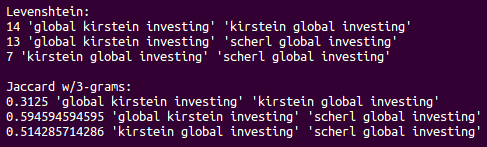
\includegraphics[width=0.9\textwidth,natwidth=1,natheight=1]{levenshtein_comp.png}
    \caption{Bad Levenstein Name Matching}
    \label{fig:lev_comp}
\end{figure}

Using levenshtein distance to match 'closest' strings, word 
inversions would be considered bulk deletions and insertions. 
The Jaccard index handels this better because inverting whole words 
still preserves the ngrams within those words even if it breaks
the joining ngrams between the words.

Admitedly, the Jaccard index is less forgiving of small typos. 
A single character edit breaks $n$ n-grams. So, for short single
word names, levenshtein distance is probably the prefered metric.

\subsection{Information Content Sensitive Jaccard Index}
The Jaccard index by itself is a fairly good way to compare names.
But it would be better if the algorithm also noticed things like
how 'unusual' certain name patterns were. 
"RJ Smith" might be closer to "CS Smith" than "RJ" based purely
on their Jaccard index, but any reasonable person would pick
"RJ Smith" and "RJ" to be the closer names because "Smith" is
such a common surname.

In more technical terms, the part of the string "Smith"
should recieve less 'weight' in the comparison function because
it conveys less information. 

Consider the more general form of the Jaccard index \cite{general}:
\begin{align*}
J(\vec{x},\vec{y}) = 
\frac{\sum_i \min(x_i, y_i)}{\sum_i \max(x_i, y_i)}
\end{align*}
Where $\vec{x}$ and $\vec{y}$ are large dimensional vectors rather 
than sets. To help relate it back to the origional form, 
imagine that $\vec{x}$ and $\vec{y}$ are lists
of counts of all the possible things that could be in the two sets
(or multisets) $A$ and $B$.
\begin{align*}
x_i = count(e_i; A)\\
e_i \in \{A \cup B \}
\end{align*}

Now if we want to consider the amount of information each little
portion of the string contains, we can calculate it
using the equation layed down by Shannon \cite{shannon}.
Namely, that the self information of an event is the log of the
inverse of the probability that event occuring. In this case,
the 'event' is the occurence of a certain n-gram in the string.

\begin{align*}
I(e_i) &= \log\left(\frac{1}{P(e_i)}\right)\\
&= -\log(P(e_i))
\end{align*}

Considering that we're searching a large sample of names, we
can get pretty close to a true approximation of the probability
of an ngram occuring in that set of names by:

\begin{align*}
P(e_i) \approx \frac{count(e_i; N)+1}{|N|+2}
\end{align*}

Where $N$ is the multiset containing the union of all the n-grams of
all the names. 
Then, we can weight the vectors $x$ and $y$ such that we have
an information sensitive comparision function: $\hat{J}(x,y)$:

\begin{align*}
\hat{J}(\vec{x},\vec{y}) &= \frac{
    \sum_i \min(x_iI(e_i), y_iI(e_i))
}{
    \sum_i \max(x_iI(e_i), y_iI(e_i))
}\\
&= J\left(\vec{x} \cdot \vec{I}, \vec{y} \cdot \vec{I} \right)\\
\vec{I} &= \left< I(e_1), I(e_2), ... I(e_n) \right>
\end{align*}

TODO: Insert Example

\section{Ambiguity}
What should the system do when the user inputs a name which is close
to the names of several entities by the chosen name comparision
function? The easiest solution would be to simply ask the user which
of the possible entities they meant. But this isn't always a great
solution; what if you're asking about a cornicopia of names?
Sure, it might be out of scope for this particular system to
resolve questions such as "Which of the actors in 'my\_data\_file.txt'
have been in movies together?" But that's certainly within the
realm of possibilities for some future work.

One approach to this problem would be to create a separate
system for distinguishing the "right" name from a small(er) selection
of possible candidates. The aformentioned Jaccard index (or similar
distance metric) might be used to narrow down the problem space
to something managable, then a much more sophisticated (yet slower)
system could choose the right name from the smaller set.

Since there are a number of string comparison algorithms, one could
(if time permited) implement several of them and use a combigned
metric to evaluate the names for fitness. For example,
a feed-forward neural net could be trained to recognize the 'right'
name based on a number of factors:
\begin{itemize}
\item String comparison functions (Jaccard, Levenshtein, etc.)
\item The self-information \cite{shannon} of the input and potential match names
\item The closeness of other potential match names
\item The prevelance of the potential match entity in the RDF data
\item The frequency of queries involving the potential match entity
\item Etc.
\end{itemize}

NOTE: I implemented just such a neural net at Discovery Data but I'm not sure how much of that system I can mention in this paper. Pybrain is an awesome library; it takes about 10 lines of code to build a working example (after coding all the factors in that list).

\bibliography{name_matching}{}
\bibliographystyle{plain}
\end{document}
